Dado que este proyecto se centrará en las bioseñales, resulta fundamental explicar los conceptos necesarios para su entendimiento. Primero se hablará brevemente sobre el procesamiento de las señales. Luego se introducirán los conceptos de extracción de características y clasificación. Finalmente, se explicará como funcionan algunos sensores y se introducirá información teórica sobre la información que se obtiene de los mismos.

\section{Procesamiento de señales}

Las señales obtenidas de los sensores poseen ruido debido a que el \emph{hardware} no es 100\% confiable. Para eliminar el ruido se utilizan tantos filtros por \emph{hardware}, que los aplica el propio sensor, y filtros por \emph{software}. Dentro de los filtros de \emph{software} se encuentra el filtro \emph{Gaussiano}. Dicho filtro suaviza la señal por lo que elimina los picos que se pudieran originar por ruido propio del sensor. Además, el filtro \emph{Gaussiano}, a diferencia de otros filtros, no elimina las altas frecuencias completamente. El filtro \emph{Gaussiano} se aplica haciendo una convolución de la señal con la siguiente función:

$$ g(x) = \frac{1}{\sqrt{2 * \pi} * \sigma } * e^{-\frac{x^{2}}{2 * \sigma^{2}}} $$

Una vez que se redujo el ruido, se pueden aplicar otros filtros o utilizarla directamente. Muchos sensores tienen como salida el nivel de potencial eléctrico medidas en $\mu V$ (microvoltios). Esta información sin ningún tipo de procesamiento no es útil. Dependiendo de que se quiera detectar se pueden realizar distintas operaciones. Una de ellas, es la búsqueda de picos. La primera derivada de un pico tiene un cruce descendente igual a cero en su máximo. Por ello, lo que se hace es primero suavizar la señal para eliminar ruido y luego se calculan las derivadas cruzadas. Luego, si la pendiente excede un umbral, significa que se ha encontrado un cero \cite{peak-finding}. Estos picos encontrados representan distintas cosas dependiendo el sensor utilizado. Por ejemplo, al utilizar un EMG, puede significar un impuslo de fuerza. En un EEG, puede significar un pestañeo.

Otro procesamiento que se le puede aplicar es la transformada discreta de \emph{Fourier}. La transformada de \emph{Fourier} transforma una función que se encuentra en el dominio del tiempo a una función que se encuentra en el dominio de la frecuencia. La transformada de \emph{Fourier} se define de la siguiente manera:

$$ x_{k} = \sum_{n=0}^{N-1} x_{n}e^{-\frac{2 \pi i}{N}kn} \qquad k = 0,\vdots, N - 1 $$

Una vez que la función se encuentra en el dominio de la frecuencia, se puede proceder con el procesamiento. Se selecciona el rango de frecuencias de interés y se le aplica un filtro pasa banda, que deja pasar un determinado rango de frecuencias de una señal y atenúa el resto. Luego de aplica el filtro pasa banda,  se cuenta con las frecuencias de interés y se continúa con el procesamiento. Una alternativa es calcular la Densidad Espectral de Potencia (DEP). Esta se define como:

$$ P = \int_{-\inf}^{+inf} S_{xx} (f) df \qquad  \textrm{donde,}$$

$$ S_{xx} = |X(f)|^{2} \qquad \textbf{y} \qquad X(f) \textrm{ es la Transformada de \emph{Fourier}} $$

Esta potencia puede ser utilizada luego como una característica de interés pero esto discutirá más adelante. Otra alternativa  es, por ejemplo, calcular el promedio de las frecuencias. Las posibilidades aquí son muchas y dependen de lo que se esté buscando.

\section{Extracción de Características de Interés y Clasificación}

Cuando se cuenta con la señal procesada, se puede utilizar directamente con reglas simples como utilizar un umbral. Este es el caso en el que se estén buscando picos. Si se buscan patrones más complejos, hay que utilizar reconocimiento de patrones. El reconocimiento de patrones tiene dos pasos principales:

\begin{itemize}
  \item \textbf{Extracción de características:} Esta etapa consiste en elegir características de la señal que sean relevantes al estado que se quiere clasificar. Por lo general estás características se colocan en un vector conocido como vector de características. El extractor utiliza como entrada una o más señales y las transforma en características útiles. Las características pueden ser por ejemplo ciertas bandas de frecuencia, calcular la DEP sobre una determinada banda de frecuencias, el valor de las derivadas en un instante del tiempo, entre otros. 
  \item \textbf{Clasificación:} En este paso se le asigna una clase a un conjunto de características (vector de características) extraído de la señal. Aquí se utilizan algoritmos de aprendizaje automático. Existen diversos algoritmos de clasificación, por ejemplo análisis discriminante lineal, árbol de decisión, clasificador bayesiano, entre otros \cite{eeg-tutorial}.
\end{itemize}

Utilizar aprendizaje automático consiste en dos etapas:

\begin{itemize}
	\item \textbf{Calibración:} Consiste en adquirir la señal de entrenamiento, optimizar las características y entrenar el clasificador. Es decir, consiste en la acumulación de datos de entrenamiento que luego son enviados al clasificador.
	\item \textbf{Uso:} Consiste en usar el modelo (características y clasificador) obtenido durante la calibración para poder reconocer el estado del usuario \cite{eeg-tutorial}. 
\end{itemize}

En el caso de utilizar un EEG para detectar si el usuario tiene los ojos cerrados, en la etapa de calibración se obtiene los datos y extraen las características deseadas y se entrena al clasificador indicando a que estado (ojos abiertos o cerrados) corresponde cada dato. Luego, en la etapa de uso, se extraen las características de la señal del usuario y se envían al clasificador para que indique en que estado se encuentra.

\begin{figure}[H]
	\centering
    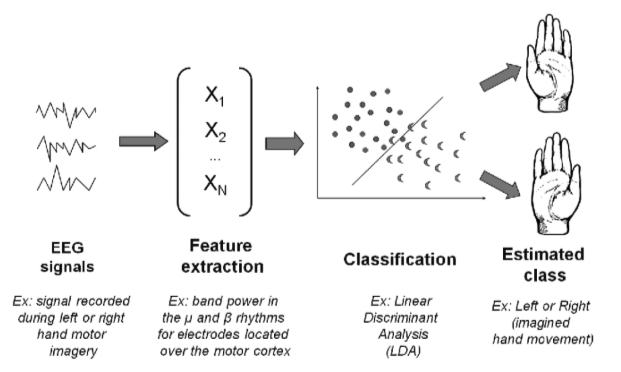
\includegraphics[width=0.8\textwidth]{eeg-pipeline.png}
    \caption{Ejemplo de las etapas por la que pasaría el procesamiento de una señal EEG \cite{eeg-tutorial}}.
	\label{fig:eeg-pipeline}
\end{figure}

En la figura \ref{fig:eeg-pipeline} se puede observar lo descripto anteriormente. Primero, se reciben las señales. Luego, se extraen las características. En este caso se trata de frecuencias asociadas a la corteza motora. Una vez que el vector de características fue creado, se envía al clasificador (en este caso análisis de discriminante lineal). Finalmente, el clasificador determina a que clase pertenece cada vector. En este ejemplo, se intento determinar si el usuario imaginó mover la mano derecha o la izquierda). 

Para medir la precisión del clasificador se arma una matriz de confusión. Ésta, es una matriz de dos dimensiones en la cuál una dimensión representa los valores actuales y otra los valores predecidos. Por ejemplo, si utilizamos el ejemplo de ojos cerrados o abiertos, la matriz se armaría de la siguiente manera:

\[
\textrm{Mat} = \begin{blockarray}{ccc}
& A & C \\
\begin{block}{c(cc)}
  A & x & y \\
  C & w & z \\
\end{block}
\end{blockarray}
 \]
 
 , donde $ A $ representa el estado de ojos abiertos y $ C $, el de ojos cerrados. La primera dimensión representa el valor obtenido y la segunda el valor predecido. Por lo tanto, $Mat_{0,0}$ representa los positivos verdaderos ($TP$) (las veces que acertó el clasificador cuando el usuario tenía los ojos abiertos), $Mat_{0,1}$ representa los falsos negativos ($FN$) (valores que el clasificador clasificó como $C$ pero en realidad era $A$), $Mat_{1,0}$ representa los falsos positivos ($FP$) (valores que el clasificador clasificó como $A$ pero en realidad era $C$), y $Mat_{1,1}$ representa los verdaderos negativos ($TN$) (valores que el clasificador clasificó como $C$ y realmente eran $C$). Utilizando esta matriz se puede obtener la precisión, la cuál se define de la siguiente manera:
 
$$ AAC = \frac{TP + TN}{P + N} $$ 
, donde $P =$ total de casos positivos y $ N =$ total de casos negativos. O simplemente:

$$ AAC = \frac{Mat_{0,0} + Mat_{1,1}}{Mat_{0,0} + Mat_{0,1} + Mat_{1,0} + Mat_{1,1}} $$ 

Los valores cercanos a $0.5$ implican que el clasificador es malo y es azar. Cuantos más cercano $1$, mejor el clasificador.
 
\section{Electroencefalograma}

Un electroencefalograma detecta la actividad eléctrica del cerebro. Estos cuentan con una determinada cantidad de electrodos que miden el nivel de potencial eléctrico en $ \mu V$. Al utilizar uno de estos dispositivos, la señal que se obtiene es el nivel de potencial eléctrico en cada electrodo. Un electroencefalograma no sirve si no se le da alguna aplicación. Aquí aparece el concepto de Interfaz Cerebro-computora (también conocido por sus silgas en inglés como BCI). "BCI es un método de comunicación basado en la actividad neuronal generada por el cerebro...El objetivo de BCI no es determinar la intensión de una persona espíando su actividad neuronal, sino que es proveer un nuevo canal de salida para el cerebro que requiere una adaptación de control voluntaria por parte del usuario"\cite{neural-eng}.

Al aplicar la Transformada de \emph{Fourier} a la señal EEG, se obtienen distintas frecuencias. En EEG, dichas frecuencias se dividen en cinco bandas:

\begin{itemize}
 \item \textbf{Alpha ($\alpha$):} $ 8 Hz \leq f \leq 13 Hz$. Las ondas Alpha se suprimen cuando los ojos se encuentran abiertos y hay estimulación visual presente. Cuando los ojos se encuentran cerrados, estas aumentan.
 \item \textbf{Beta ($\beta$):} $ 13 Hz \leq f \leq 30 Hz$. Las ondas Beta se asocian la concentración.
 \item \textbf{Delta ($\delta$):} $ 0.5 Hz \leq f \leq 4 Hz$. Estas ondas aparecen en etapas de sueño profundo.
 \item \textbf{Theta ($\theta$):} $ 4 Hz \leq f \leq 8 Hz$. Las ondas Theta aparecen en las primeras etapas de sueño.
 \item \textbf{Gamma ($\gamma$):} $ 30 Hz \leq f \leq 60 Hz$. Las ondas Gamma aparecen cuando hay un aumento de la actividad mental cognitiva \cite{neural-eng}.
\end{itemize}

\section{EMG}

\section{EKG}